\documentclass[11pt]{article}

\usepackage[a4paper,margin=1in]{geometry}
\usepackage{lmodern}
\usepackage{microtype}
\usepackage{amsmath,amssymb}
\usepackage{booktabs}
\usepackage{array}
\usepackage{siunitx}
\usepackage{hyperref}
\usepackage{tikz}
\usepackage{pgfplots}
\usepackage{pgfplotstable}
\usepackage{xcolor}

\pgfplotsset{compat=1.18}
\sisetup{detect-all}
\hypersetup{colorlinks=true,linkcolor=blue!50!black,citecolor=blue!50!black,urlcolor=blue!50!black}
\usetikzlibrary{arrows.meta,positioning,fit,calc}

\title{Controllable Neural Cellular Automata for Periodic Maze Navigation with Terminal Lockout}
\author{nca-control project}
\date{March 30, 2026}

\begin{document}
\maketitle

\begin{abstract}
This report summarizes the current state of a research implementation of controllable neural cellular automata (NCA) for a discrete two-dimensional control task. The target environment is a periodic grid containing empty cells, blocked cells, a single controllable active cell, and an exit condition that triggers irreversible terminal dynamics. The implementation combines an exact deterministic reference engine, supervised one-step learning, automated rollout evaluation, a browser-based interactive visualizer, and two learning backends: PyTorch and MLX. The main empirical finding is that, under a stronger MLX training protocol, the smallest exact and reproducible model discovered so far uses 12 hidden channels with a \(3\times 3\) perception kernel and a \(1\times 1\) update kernel. This model remains exact on larger unseen grids up to \(200\times 200\) in the recorded validation runs. A recent maintenance pass preserved these results on the current code base and confirmed that the selected model still reproduces on a known-good seed.
\end{abstract}

\paragraph{Provenance.}
The contents of this project are AI generated. The implementation, documentation, and experimental write-up were produced with OpenAI Codex using the GPT-5.4 model with High reasoning effort.

\section{Introduction}
Neural cellular automata study how spatially shared local update rules can generate or maintain structured global behavior. In the present project, the focus is narrower and control-oriented: instead of image growth or regeneration alone, the learned local rule must emulate a deterministic game-like transition system driven by user actions. The task is intentionally minimal but exacting. The system must preserve exactly one active cell, respect walls, wrap around periodic boundaries, stop responding after an exit state is reached, and propagate a terminal fill state over time.

The project evolved stepwise from a plain periodic movement task to a wall-aware maze task and then to an exit-aware maze task. Along the way, the implementation acquired automated tests, text-mode simulation, browser-based interactive verification, exact rollout evaluation, throughput instrumentation, and an alternative MLX backend for Apple Silicon. The central question at the current stage is no longer whether the task can be solved, but how small and how reproducible the learned local rule can be.

\section{Task Definition}
Let the grid domain be the discrete torus
\[
\Lambda_{H,W} = \mathbb{Z}_H \times \mathbb{Z}_W.
\]
At time \(t\), the deterministic \texttt{maze\_exit} state can be written as
\[
s_t = (p_t, B, x, F_t, \tau_t),
\]
where \(p_t \in \Lambda_{H,W}\) is the active-cell position when the system is non-terminal, \(B \subset \Lambda_{H,W}\) is the set of blocked cells, \(x \in \Lambda_{H,W}\) is the maze exit, \(F_t \subseteq \Lambda_{H,W}\) is the exit-fill set, and \(\tau_t \in \{0,1\}\) is the terminal flag.

The action alphabet is
\[
\mathcal{A} = \{\texttt{none}, \texttt{up}, \texttt{down}, \texttt{left}, \texttt{right}\}.
\]
Before termination, the active cell proposes a one-step move according to the input action and periodic boundary conditions. If the target cell is blocked, the move is cancelled. If the target cell is the exit, the system becomes terminal. After termination, future actions are ignored, the active cell disappears, and the exit-fill state expands deterministically over subsequent clock ticks until the accessible region is filled.

\paragraph{Cell semantics.}
The current implementation distinguishes four semantic cell types:
\begin{enumerate}
  \item empty cells, over which movement is allowed;
  \item blocked cells, which act as walls;
  \item a single active cell, controlled by the input action;
  \item exit-fill cells, which denote terminal spread after the active cell reaches the exit.
\end{enumerate}

\begin{table}[t]
\centering
\caption{Semantic components of the implemented task.}
\begin{tabular}{>{\raggedright\arraybackslash}p{0.20\linewidth} >{\raggedright\arraybackslash}p{0.70\linewidth}}
\toprule
Component & Behavior \\
\midrule
Periodic boundary & Motion wraps on all four boundaries. \\
Blocked cells & Static walls; attempted moves into walls are cancelled. \\
Active cell & Exactly one cell before termination; moved by the action input. \\
Exit cell & Static goal generated by the maze constructor. \\
Terminal lockout & Once the exit is reached, later actions have no effect. \\
Exit-fill dynamics & The terminal color spreads deterministically after termination. \\
\bottomrule
\end{tabular}
\end{table}

\section{Implementation}
\subsection{Reference system}
The project maintains a deterministic Python reference engine that defines the target dynamics exactly. This engine is used for:
\begin{itemize}
  \item dataset generation,
  \item text-mode simulation,
  \item rollout verification,
  \item browser-side comparison against the learned model.
\end{itemize}
The maze generator itself is not learned. It is a pure Python component that produces solvable mazes with designated start and exit cells, and the browser visualizer generates a fresh maze on reset.

\subsection{Learned local rule}
The learned model is deliberately small and strictly local. For the current \texttt{maze\_exit} task, the input channels are:
\begin{itemize}
  \item active-cell channel,
  \item exit-fill channel,
  \item blocked-cell channel,
  \item five action channels corresponding to \(\mathcal{A}\).
\end{itemize}
Thus the model consumes eight channels and predicts two output channels (active and exit-fill).

Let \(u_t\) denote the stacked input tensor at time \(t\). The learned update path has the form
\begin{align*}
h_t &= \mathrm{ReLU}\!\left(\mathrm{Conv}^{\mathrm{circ}}_{k_p}(u_t)\right), \\
z_t &= \mathrm{ReLU}\!\left(\mathrm{Conv}^{\mathrm{circ}}_{k_u}(h_t)\right), \\
\hat{y}_t &= \mathrm{Conv}_{1\times 1}(z_t),
\end{align*}
with circular padding so that the learned rule is compatible with periodic boundaries. For \texttt{maze\_exit}, the raw output is squashed channelwise and then decoded back to a valid gameplay state during evaluation and visualization.

\begin{figure}[t]
\centering
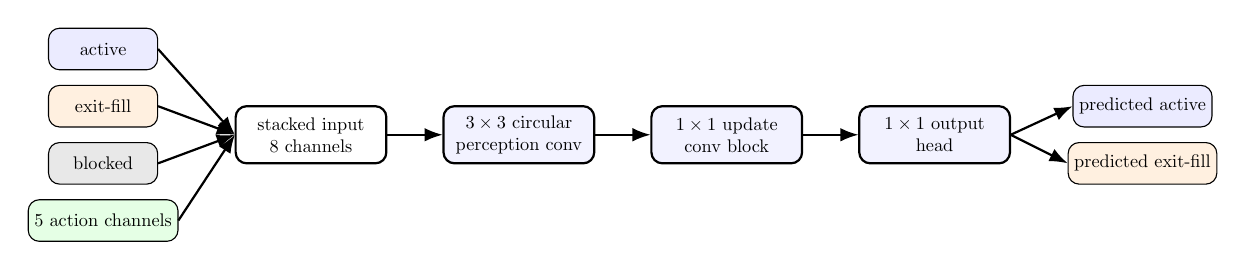
\begin{tikzpicture}[
    scale=0.66,
    transform shape,
    box/.style={draw, rounded corners, thick, align=center, minimum width=2.9cm, minimum height=1.1cm},
    smallbox/.style={draw, rounded corners, align=center, minimum width=2.1cm, minimum height=0.8cm},
    >=Latex
]
  \node[smallbox, fill=blue!8] (active) at (0,1.3) {active};
  \node[smallbox, fill=orange!12] (fill) at (0,0.2) {exit-fill};
  \node[smallbox, fill=gray!18] (blocked) at (0,-0.9) {blocked};
  \node[smallbox, fill=green!10] (action) at (0,-2.0) {5 action channels};
  \node[box, fill=white] (stack) at (4.0,-0.35) {stacked input\\\(8\) channels};
  \node[box, fill=blue!5] (conv1) at (8.0,-0.35) {\(3\times 3\) circular\\perception conv};
  \node[box, fill=blue!5] (conv2) at (12.0,-0.35) {\(1\times 1\) update\\conv block};
  \node[box, fill=blue!5] (out) at (16.0,-0.35) {\(1\times 1\) output\\head};
  \node[smallbox, fill=blue!8] (preda) at (20.0,0.2) {predicted active};
  \node[smallbox, fill=orange!12] (predf) at (20.0,-0.9) {predicted exit-fill};

  \draw[->, thick] (active.east) -- (stack.west);
  \draw[->, thick] (fill.east) -- (stack.west);
  \draw[->, thick] (blocked.east) -- (stack.west);
  \draw[->, thick] (action.east) -- (stack.west);
  \draw[->, thick] (stack.east) -- (conv1.west);
  \draw[->, thick] (conv1.east) -- (conv2.west);
  \draw[->, thick] (conv2.east) -- (out.west);
  \draw[->, thick] (out.east) -- (preda.west);
  \draw[->, thick] (out.east) -- (predf.west);
\end{tikzpicture}
\caption{Current learned transition pipeline for the \texttt{maze\_exit} task. The same local rule is applied at every grid location.}
\label{fig:pipeline}
\end{figure}

\subsection{Software backends}
The repository retains both a PyTorch implementation and an MLX implementation. PyTorch remains useful for CPU execution and future CUDA-class hardware, while MLX is currently the preferred Apple Silicon backend. The implementation also includes:
\begin{itemize}
  \item a text-based simulation interface for scripted testing,
  \item one-step evaluation scripts,
  \item rollout evaluation scripts,
  \item a browser-based interactive visualizer with a fixed simulation clock.
\end{itemize}

\section{Experimental Protocol}
The project progressed through multiple experimental phases:
\begin{enumerate}
  \item plain periodic active-cell control;
  \item wall-aware maze control;
  \item exit-aware maze control with terminal fill;
  \item backend comparison (PyTorch CPU, PyTorch MPS, MLX);
  \item minimal-model sweeps under increasingly stronger training budgets;
  \item post-selection large-grid validation and maintenance reruns.
\end{enumerate}

The current minimal-model result is based on the strongest search protocol used so far:
\begin{itemize}
  \item backend: MLX;
  \item task: \texttt{maze\_exit};
  \item training grid: \(9\times 9\);
  \item training mazes: \(64\);
  \item epochs: \(300\);
  \item batch size: \(128\);
  \item candidate widths: \(8, 9, 10, 11, 12,\dots\);
  \item reproducibility seeds: \(0,1,2,3\).
\end{itemize}

Acceptance required exact one-step behavior together with exact rollout behavior on held-out larger grids. A later validation pass extended rollout checks to \(100\times 100\) and \(200\times 200\) grids.

\section{Results}
\subsection{Backend comparison}
On the benchmarked \(9\times 9\) workload, MLX clearly dominated the measured training throughput on Apple Silicon, while PyTorch MPS lagged behind both MLX and CPU for this small-scale regime. Figure~\ref{fig:backend} reports the recorded throughput values from the fixed benchmark run.

\begin{figure}[t]
\centering
\begin{tikzpicture}
\begin{axis}[
    width=0.78\linewidth,
    height=6cm,
    ybar,
    bar width=16pt,
    ymin=0,
    ylabel={samples/s},
    symbolic x coords={PyTorch CPU,PyTorch MPS,MLX},
    xtick=data,
    xticklabel style={rotate=20,anchor=east},
    nodes near coords,
    every node near coord/.append style={font=\small, rotate=90, anchor=west},
    enlarge x limits=0.25,
    axis lines*=left,
]
\addplot[fill=blue!45] table[x=backend,y=samples_per_second,col sep=comma] {data/backend_benchmark.csv};
\end{axis}
\end{tikzpicture}
\caption{Measured training throughput on the fixed \(9\times 9\) backend benchmark. MLX was the fastest backend on the tested Apple Silicon machine.}
\label{fig:backend}
\end{figure}

\subsection{Minimal-model search}
Earlier weaker training budgets yielded a \(32/3/1\) model as the smallest working architecture. After moving to MLX and strengthening the training protocol, the minimal exact model dropped to \(12/3/1\). Tight boundary checks then showed that nearby smaller models still fail:
\begin{itemize}
  \item \(9/3/1\): screening success, but failed reproducibility;
  \item \(10/3/1\): failed screening;
  \item \(11/3/1\): screening success, but failed reproducibility;
  \item \(12/3/1\): exact and reproducible on the tested seed set.
\end{itemize}

\begin{table}[t]
\centering
\caption{Tight minimal-model boundary check under the strong MLX protocol.}
\begin{tabular}{ccccccc}
\toprule
Hidden & One-step & \(30\times 30\) & \(50\times 50\) & Repro attempts & Repro passes & Status \\
\midrule
9  & 1.0000 & 1.0000 & 1.0000 & 2 & 1 & failed \\
10 & 0.8626 & 0.0000 & 0.0000 & 0 & 0 & failed \\
11 & 1.0000 & 1.0000 & 1.0000 & 4 & 3 & failed \\
12 & 1.0000 & 1.0000 & 1.0000 & 4 & 4 & selected \\
\bottomrule
\end{tabular}
\label{tab:minimal}
\end{table}

\begin{figure}[t]
\centering
\begin{tikzpicture}
\begin{axis}[
    width=0.78\linewidth,
    height=6cm,
    ymin=0,
    ymax=1.05,
    xlabel={hidden channels},
    ylabel={accuracy / pass fraction},
    xtick=data,
    legend style={at={(0.5,-0.23)},anchor=north,legend columns=2},
    axis lines*=left,
]
\addplot+[mark=o, thick, blue] table[x=hidden_channels,y=screen_full_state_accuracy,col sep=comma] {data/minimal_candidates.csv};
\addlegendentry{screen one-step}
\addplot+[mark=square*, thick, orange] table[x=hidden_channels,y=repro_pass_fraction,col sep=comma] {data/minimal_candidates.csv};
\addlegendentry{repro pass fraction}
\end{axis}
\end{tikzpicture}
\caption{Boundary behavior near the selected minimal model. Width 12 is the smallest candidate that passed the tested reproducibility gate.}
\label{fig:minimal}
\end{figure}

\subsection{Training dynamics and maintenance rerun}
The recent maintenance pass was important because it modified shared movement logic and aligned the documentation with the code base. After that refactor, the full automated suite still passed (\(62\) tests passed and one MLX-specific test remained skipped in the default sandboxed run), and a clean seed-0 MLX rerun reproduced the exact regime.

Figure~\ref{fig:loss} contrasts the clean seed-0 rerun against an exploratory seed-4 run. The seed-0 curve descends into the same low-loss regime recorded during the original reproducibility study, while the seed-4 curve plateaus much higher. This does not invalidate the selected model, but it does show that convergence is not guaranteed for arbitrary new seeds under the present recipe.

\begin{figure}[t]
\centering
\begin{tikzpicture}
\begin{semilogyaxis}[
    width=0.82\linewidth,
    height=6.5cm,
    xlabel={epoch},
    ylabel={training loss},
    legend style={at={(0.5,-0.23)},anchor=north,legend columns=2},
    axis lines*=left,
]
\addplot[thick, blue] table[x=epoch,y=loss,col sep=comma] {data/loss_seed0_rerun.csv};
\addlegendentry{seed 0 rerun}
\addplot[thick, red!75!black] table[x=epoch,y=loss,col sep=comma] {data/loss_seed4_exploratory.csv};
\addlegendentry{seed 4 exploratory}
\end{semilogyaxis}
\end{tikzpicture}
\caption{Training-loss traces for the fresh seed-0 rerun and exploratory seed-4 run. The plotted CSV is generated from recorded progress artifacts.}
\label{fig:loss}
\end{figure}

\subsection{Generalization to larger grids}
The strongest current evidence for scale robustness is that the selected \(12/3/1\) model remained exact on larger unseen grids in the recorded validation experiments. This follows both from the multi-seed validation documented for seeds \(0\) through \(3\), and from the recent fresh seed-0 rerun on the current code base.

\begin{table}[t]
\centering
\caption{Fresh post-maintenance verification of the selected \(12/3/1\) model on a clean seed-0 retrain.}
\begin{tabular}{lccc}
\toprule
Evaluation & Grid & Rollout setting & Result \\
\midrule
One-step evaluation & \(9\times 9\) & held-out generated mazes & full-state accuracy \(=1.0\) \\
Rollout evaluation & \(50\times 50\) & 32 sequences, 200 steps & exact rollout rate \(=1.0\) \\
Rollout evaluation & \(100\times 100\) & 32 sequences, 200 steps & exact rollout rate \(=1.0\) \\
Rollout evaluation & \(200\times 200\) & 16 sequences, 200 steps & exact rollout rate \(=1.0\) \\
\bottomrule
\end{tabular}
\label{tab:generalization}
\end{table}

\section{Discussion}
Three conclusions are currently well supported by the implementation and experiments.

First, the task itself is local enough to be captured by a small shared convolutional rule. This is consistent with the design of the deterministic environment: motion, blocking, exit detection, and terminal spread all depend on local neighborhoods and a small amount of persistent state.

Second, backend choice matters substantially on Apple Silicon. For the current workload, MLX made it practical to run stronger architecture sweeps and reproducibility studies than were previously reasonable under PyTorch MPS.

Third, the present model should be described as \emph{reproducible on the tested seed set}, not as universally seed-invariant. The recorded evidence is strong for seeds \(0\) through \(3\), and the maintenance rerun reconfirmed seed \(0\) on the current code base. However, the exploratory seed-4 run demonstrates that a fresh initialization can still fail to reach the exact regime.

Two limitations are important. The learned system is not solving maze planning; it is learning the transition law conditioned on external actions. In addition, the deferred patch-local training idea has not yet been implemented, so the current report only covers full-state supervised training.

\section{Conclusion}
The project now contains a verified controllable NCA-style implementation for periodic maze navigation with walls, terminal exit lockout, and autonomous exit-fill dynamics. The software stack includes deterministic reference dynamics, automated tests, browser-based interactive verification, PyTorch and MLX backends, architecture sweep tooling, and reproducibility-oriented evaluation.

The main empirical conclusion is that the currently smallest exact and reproducible model discovered so far is a \(12/3/1\) architecture trained with MLX under a stronger \(9\times 9\), 64-maze, 300-epoch protocol. This model remained exact on substantially larger grids in the recorded validation runs and survived a clean post-maintenance regression rerun on a known-good seed. The immediate next research question is whether an even more local training formulation, such as patch-based supervision, can preserve these guarantees while further reducing training cost.

\begin{thebibliography}{9}

\bibitem{mordvintsev2020growing}
Alexander Mordvintsev, Ettore Randazzo, Eyvind Niklasson, and Michael Levin.
\newblock Growing Neural Cellular Automata.
\newblock \emph{Distill}, 2020.
\newblock DOI: 10.23915/distill.00023.

\bibitem{gilpin2019ca}
William Gilpin.
\newblock Cellular automata as convolutional neural networks.
\newblock \emph{Physical Review E}, 100(3):032402, 2019.
\newblock DOI: 10.1103/PhysRevE.100.032402.

\bibitem{paszke2019pytorch}
Adam Paszke et al.
\newblock PyTorch: An Imperative Style, High-Performance Deep Learning Library.
\newblock In \emph{Advances in Neural Information Processing Systems 32}, pages 8024--8035, 2019.

\bibitem{mlx2023}
Awni Hannun, Jagrit Digani, Angelos Katharopoulos, and Ronan Collobert.
\newblock MLX: Efficient and flexible machine learning on Apple silicon.
\newblock Software citation provided by the official MLX project, 2023.
\newblock \url{https://github.com/ml-explore/mlx}.

\bibitem{wolfram1983statistical}
Stephen Wolfram.
\newblock Statistical mechanics of cellular automata.
\newblock \emph{Reviews of Modern Physics}, 55(3):601--644, 1983.

\end{thebibliography}

\end{document}
